\problemset{Теория вероятностей и математическая статистика}
\problemset{Индивидуальное домашнее задание №2}
\problemset{Вариант №21}

\renewcommand*{\proofname}{Решение}

\begin{problem}
	На плоскости расчерчена прямоугольная сетка, величина ячейки 9 $\times$ 8 единиц. Определить вероятность того, что монета диаметра 4, наугад брошенная на плоскость, не пересечёт ни одной прямой.
\end{problem}

\begin{proof}
	Представим событие A - монета не пересечёт сетки в виде двух событий: B - монета не пересечёт вертикальных линий и C - монета не пересечёт горизонтальных линий. Тогда $P(A) = P(B) \cdot P(C)$.
	\newline
	Вероятность попадания монеты на параллельные прямые равна вероятности попадания центра монеты в область, находящуюся от любой прямой на расстоянии, большем, чем радиус монеты, делённой на вероятность попадания центра монеты в область между прямыми:
	\[
		P(X) = \frac{a - d}{a}
	\]
	, где a - расстояние между прямыми, а d - диаметр монеты.
	\newline
	Таким образом мы можем высчитать вероятности событий B и C, а, следовательно, и события A:
	\[
		P(A) = P(B) \cdot P(C) = \frac{9 - 4}{9} \cdot \frac{8 - 4}{8} = \frac{5}{9} \cdot \frac{4}{8} = \frac{5}{18}
	\]
	Ответ: $\frac{5}{18}$.
\end{proof}

\begin{problem}
	Дана функция распределения случайной величины $\xi$:
	$\begin{matrix}
		x & (-\infty,0] & (0,3] & (3,\infty)\\
		F_\xi(x) & 0 & \frac{2}{3} & 1
	\end{matrix}$. Вычислить \textbf{E}$\xi$, \textbf{D}$\xi$, энтропию $\xi$ и распределение $\eta = \xi^4$.
\end{problem}

\begin{proof}
	Построим график функции распределения $\xi$:
	\begin{center}
		\begin{tikzpicture}
			\begin{axis}[
				xmin=-3, xmax=6,
				ymin=-1, ymax=2,
				axis lines=middle,
				xlabel=$x$,
				ylabel=$y$
			]
				\addplot [color=black, line width=3pt] coordinates {(-4, 0)(0, 0)};
				\addplot [color=black, line width=3pt] coordinates {(0, 2/3)(3, 2/3)};
				\node[circle, draw=black, fill=white, scale=1] at (axis cs: 0, 2/3) {};
				\addplot [color=black, line width=3pt] coordinates {(3, 1)(7, 1)};
				\node[circle, draw=black, fill=white, scale=1] at (axis cs: 3, 1) {};
			\end{axis}
		\end{tikzpicture}
	\end{center}
	Найдём закон распределения $\xi$, разделив функцию на отрезки:
	\begin{center}
		\begin{tabular}{|c||c|c|}
			\hline
			x & 0 & 3 \\
			\hline
			p & 2/3 & 1/3 \\
			\hline
		\end{tabular}
	\end{center}
	Проверим верность построения: $\sum p_n = 1$.
	\newline
	Рассчитаем математическое ожидание, для дискретной случайной величины оно вычисляется по формуле $\textbf{E}\xi = \sum_{i = 1}^{n} x_i \cdot p_i$:
	\[
		\textbf{E}\xi = (0 \cdot \frac{2}{3}) + (3 \cdot \frac{1}{3}) = 1
	\]
	Рассчитаем дисперсию, $\textbf{D}\xi = \textbf{E}(\xi - \textbf{E}\xi)^2$. Для этого добавим в таблицу законна распределения ещё одну вспомогательную строку:
	\begin{center}
		\begin{tabular}{|c||c|c|}
			\hline
			x & 0 & 3 \\
			\hline
			p & 2/3 & 1/3 \\
			\hline
			$(x - \textbf{E}\xi)^2$ & 1 & 4 \\
			\hline
		\end{tabular}
	\end{center}
	Для дискретной случайной величины она вычисляется по формуле $\textbf{D}\xi = \sum_{i = 1}^{n} (x_i - \textbf{E}\xi)^2 \cdot p_i$:
	\[
		\textbf{D}\xi = (1 \cdot \frac{2}{3}) + (4 \cdot \frac{1}{3}) = 2
	\]
	Проверим верность вычисления: $\textbf{D}\xi > 0$.
	\newline
	Рассчитаем энтропию, для дискретной случайной величины она вычисляется по формуле $\textbf{H}\xi = -\sum_{i = 1}^{n} p_i \cdot \log(p_i)$:
	\[
		\textbf{H}\xi = (\frac{2}{3} \cdot \log(\frac{2}{3})) + (\frac{1}{3} \cdot \log(\frac{1}{3})) \eqcirc -0.27643
	\]
	Найдём закон распределения случайной величины $\eta = \xi^4$:
	\begin{center}
		\begin{tabular}{|c||c|c|}
			\hline
			x & 0 & 27 \\
			\hline
			p & 2/3 & 1/3 \\
			\hline
		\end{tabular}
	\end{center}
	Следовательно, $F_\eta(x)=
	\begin{dcases}
		0, \; -\infty < x \leq 0\\
		2/3, \; 0 < x \leq 27\\
		1, \; 27 < x < \infty
	\end{dcases}$. Построим график функции распределения $\eta$:
	\begin{center}
		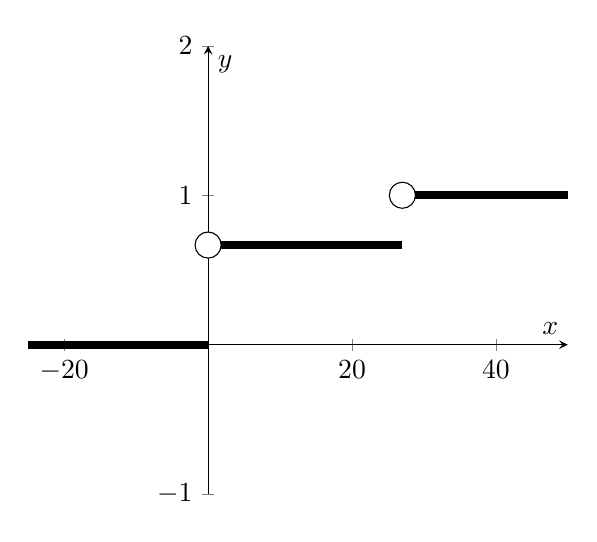
\begin{tikzpicture}
			\begin{axis}[
				xmin=-25, xmax=50,
				ymin=-1, ymax=2,
				axis lines=middle,
				xlabel=$x$,
				ylabel=$y$
			]
				\addplot [color=black, line width=3pt] coordinates {(-26, 0)(0, 0)};
				\addplot [color=black, line width=3pt] coordinates {(0, 2/3)(27, 2/3)};
				\node[circle, draw=black, fill=white, scale=1] at (axis cs: 0, 2/3) {};
				\addplot [color=black, line width=3pt] coordinates {(27, 1)(51, 1)};
				\node[circle, draw=black, fill=white, scale=1] at (axis cs: 27, 1) {};
			\end{axis}
		\end{tikzpicture}
	\end{center}
\end{proof}

\begin{problem}
	Дана плотность распределения абсолютно непрерывной случайной величины $\xi$: $p(x)=
	\begin{dcases}
		C|x|, \; x \in [-\pi;\frac{2}{3}\pi]\\
		0, \; x \notin [-\pi;\frac{2}{3}\pi]
	\end{dcases}$. Вычислить C, \textbf{E}$\xi$, \textbf{D}$\xi$, энтропию $\xi$ и распределение $\eta = \cos(3\xi)$.
\end{problem}

\begin{proof}
	Известно, что функция распределения $F'(x) = p(x)$. Следовательно, $F_\xi(x) =
	\begin{dcases}
		0, \; x \in (-\infty;-\pi]\\
		g(x), \; x \in [-\pi;\frac{2}{3}\pi]\\
		1, \; x \notin [\frac{2}{3}\pi;\infty]
	\end{dcases}$, где $g(x) = \int C|x| dx$ такая, что $g(-\pi) = 0$ и $g(\frac{2}{3}\pi) = 1$ (из-за непрерывности $\xi$).
	\newline
	Вычислим С по формуле $\int_{-\infty}^{\infty} p(x) dx = 1$:
	\[
		\int_{-\infty}^{\infty} p(x) dx = \int_{-\infty}^{-\pi} 0 dx + \int_{-\pi}^{\frac{2}{3}\pi} C|x| dx + \int_{\frac{2}{3}\pi}^{\infty} 0 dx = \int_{-\pi}^{\frac{2}{3}\pi} C|x| dx = C \cdot \frac{13}{18}\pi^2 = 1
	\]
	Следовательно, $C = \frac{18}{13\pi^2} \approx 0.44074$.
	\newline
	Построим график плотности распределения $\xi$:
	\begin{center}
		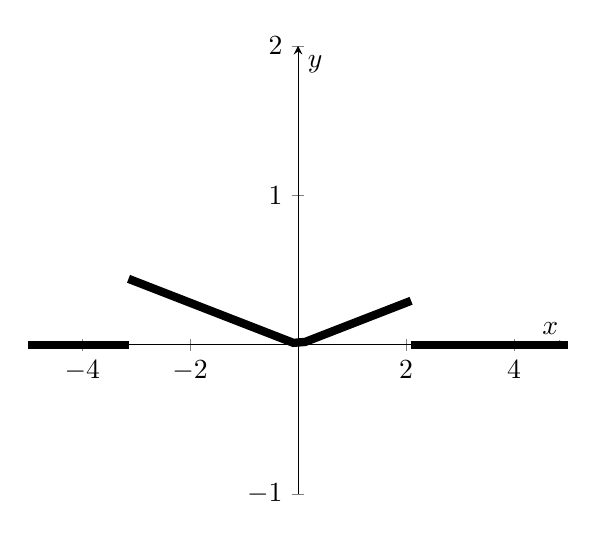
\begin{tikzpicture}
			\begin{axis}[
				xmin=-5, xmax=5,
				ymin=-1, ymax=2,
				axis lines=middle,
				xlabel=$x$,
				ylabel=$y$
			]
				\addplot [color=black, line width=3pt] coordinates {(-6, 0)(-pi, 0)};
				\addplot [color=black, line width=3pt, domain=-pi:2*pi/3] {18/(13*pi^2) * abs(x)};
				\addplot [color=black, line width=3pt] coordinates {(2*pi/3, 0)(6, 0)};
			\end{axis}
		\end{tikzpicture}
	\end{center}
	Найдём функцию распределения $\xi$:
	\[
		F_\xi(x) = \int_{-\pi}^{\frac{2}{3}\pi} \frac{18}{13\pi^2} |x| dx = \frac{18}{26\pi^2} x^2 \cdot sign(x) + const.
	\]
	Подставим точку $(-\pi, 0)$, чтобы узнать константу:
	\[
		\frac{18}{26\pi^2} (-\pi)^2 \cdot (-1) + const. = 0
	\]
	Следовательно, $const. = \frac{9}{13}$.
	\newline
	Построим график функции распределения $\xi$:
	\begin{center}
		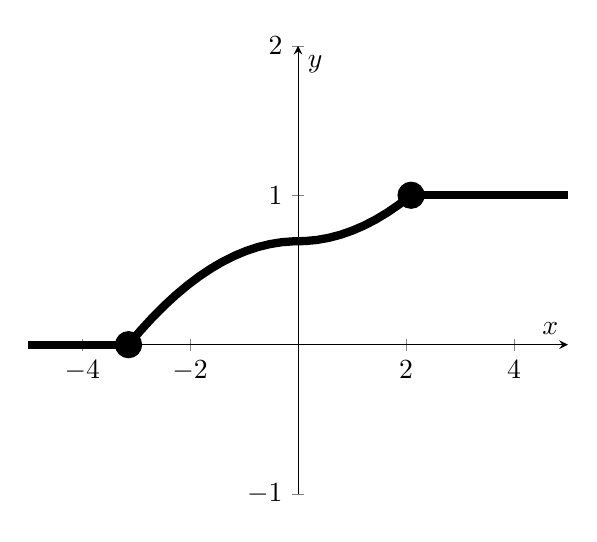
\begin{tikzpicture}
			\begin{axis}[
				xmin=-5, xmax=5,
				ymin=-1, ymax=2,
				axis lines=middle,
				xlabel=$x$,
				ylabel=$y$
			]
				\addplot [color=black, line width=3pt] coordinates {(-6, 0)(-pi, 0)};
				\node[circle, draw=black, fill=black, scale=1] at (axis cs: -pi, 0) {};
				\addplot [color=black, line width=3pt, domain=-pi:2*pi/3] {18/(26*pi^2) * x*abs(x) + 9/13};
				\node[circle, draw=black, fill=black, scale=1] at (axis cs: 2*pi/3, 1) {};
				\addplot [color=black, line width=3pt] coordinates {(2*pi/3, 1)(6, 1)};
			\end{axis}
		\end{tikzpicture}
	\end{center}
	Рассчитаем математическое ожидание, для непрерывной случайной величины оно вычисляется по формуле $\textbf{E}\xi = \int x p(x) dx$:
	\[
		\textbf{E}\xi = \int_{-\pi}^{\frac{2}{3}\pi} \frac{18}{13\pi^2} x^2 dx = -\frac{38\pi}{117} \approx -1.02035
	\]
	Рассчитаем дисперсию по формуле $\textbf{D}\xi = \int x^2 p(x) dx - {\textbf{E}\xi}^2$:
	\[
		\textbf{D}\xi = \int_{-\pi}^{\frac{2}{3}\pi} \frac{18}{13\pi^2} x^2 |x| dx - {\textbf{E}\xi}^2 = \frac{97}{234} \pi^2 - \frac{1444}{13689} \pi^2 = \frac{8461}{27378} \pi^2 \approx 3.05014
	\]
	Проверим верность вычисления: $\textbf{D}\xi > 0$.
	Рассчитаем энтропию, для непрерывной случайной величины она вычисляется по формуле $\textbf{H}\xi = -\int p(x) \log(p(x)) dx$:
	\[
		\textbf{H}\xi = -\int_{-\pi}^{\frac{2}{3}\pi} \frac{18}{13\pi^2} |x| \cdot \log(\frac{18}{13\pi^2} |x|) dx = log(\frac{6 \cdot 2^{\frac{4}{13}} \cdot 3^{\frac{9}{13}}}{13\pi}) - \frac{1}{2} \approx -1.4441
	\]
	Найдём функцию распределения случайной величины $\eta$:
	\[
		F_\eta(x) = p(\eta < x) = p(\cos(3\xi) < x) = p(\xi < \frac{\arccos(x)}{3}) = F_\xi(\frac{\arccos(x)}{3})
	\]
	Следовательно, подставив крайние значения $F_\xi(x)$ в уравнение $\eta$, получим:
	\[F_\eta(x) =
	\begin{dcases}
	0, \; x \in (-\infty;-1]\\
	\frac{6}{26\pi^2} \arccos(x)^2 \cdot sign(x) + \frac{9}{13}, \; x \in [-1;1]\\
	1, \; x \notin [1;\infty]
	\end{dcases}
	\]
\end{proof}